%% Copyright 1998 Pepe Kubon
%%
%% `two.tex' --- 2nd chapter for thes-full.tex, thes-short-tex from
%%               the `csthesis' bundle
%%
%% You are allowed to distribute this file together with all files
%% mentioned in READ.ME.
%%
%% You are not allowed to modify its contents.
%%

%%%%%%%%%%%%%%%%%%%%%%%%%%%%%%%%%%%%%%%%%%%%%%%%%
%
%     Chapter 4  
%
%%%%%%%%%%%%%%%%%%%%%%%%%%%%%%%%%%%%%%%%%%%%%%%%

\chapter{A Pruning-based Method on Graphs}
\label{ch:graph}

In this chapter, we will introduce the algorithms to compute the skyline subspace queries. One naive way to solve this problem is to compute the labeled distance vectors of all the vertices first and enumerate all subspaces to check whether the query vertex is a subspace skyline in those subspaces using the existing skyline computation algorithms. Given a label graph $G=(V, E, L)$, the time complexity of this method is $O((|V|+|E|)|L| + 2^{|L|}|L||V|^2)$. $O((|V|+|E|)|L|)$ is the complexity to traverse the whole graph to get \emph{labeled distance vectors} of all vertices. $O(2^{|L|})$ is the complexity of enumerating every subspace of a $|L|$-dimensional space. $O(|L||V|^2)$ is the time complexity of computing the skyline points in one particular subspace. This brute force method is very time consuming. In order to make the algorithm more efficient, we propose a bottom-up set enumeration algorithm and manage to avoid some unnecessary computation by applying some pruning techniques in our method.

\begin{table}[h]
\centering
\begin{tabular}{|l|p{11cm}|}
\hline
Symbol                      & Interpretation                                                                                                                                     \\ \hline
$q$                         & query vertex $q$                                                                                                                                   \\ \hline
$LV_v$                      & labeled distance vector of vertex $v$ representing the distances between $v$ and each label.                                                         \\ \hline
$\mathcal{B}$               & subspace $\mathcal{B}$                                                                                                                             \\ \hline
$\mathit{SDS}_u$            & strictly dominating subspace of $u$                                                                                                                \\ \hline
$\mathit{EQ}_u$             & equivalence subspace of $u$                                                                                                                        \\ \hline
$\mathit{CAND}_\mathcal{B}$ & dominating candidate set of subspace $\mathcal{B}$                                                                                                 \\ \hline
$(u, dom)$                  & element in dominating candidate set. $(u, dom) \in \mathit{CAND}_\mathcal{B}$ means that $u$ dominates query vertex $q$ in subspace $\mathcal{B}$. \\ \hline
$(u, eq)$                   & element in dominating candidate set. $(u, eq) \in \mathit{CAND}_\mathcal{B}$ means that $u$ dominates query vertex $q$ in subspace $\mathcal{B}$.  \\ \hline
\end{tabular}
    \caption{Symbols Used in the Pruning-based Method on Graph}
    \label{tab:symbol_graph}
\end{table}

\section{BFS Label Collecting}
\label{sec:bfs-collect}
We collect the $d$-hop labels using Breadth-First-Search and get the \emph{labeled distance vector} of the the query vertex. The idea is that we start with the query vertex and traverse the graph in a breadth first manner. If we visit a vertex with a new label that we have not visited before, we update the corresponding entry of that label in the \emph{labeled distance vector} to the distance from the query vertex. The Breadth First Search process will end if all reachable vertices in up to $d$ hops have been visited. Then we will get the \emph{labeled distance vector} of the query vertex when the BFS label collecting ends. Algorithm~\ref{algo:graph_collect} shows the process of label collecting.

\begin{algorithm}[h]
  \caption{Label Collecting}
  \label{algo:graph_collect}
  \begin{algorithmic}[1]
  \show\LOOP
    \REQUIRE A graph $G=(V,E)$, a list of label sets $F=\left\{L_v | v \in V\right\}$, the label sets of all vertices, a query vertex $q$, the number of hops $d$;
    \ENSURE The labeled distance vector $LV_q$ of the query vertex $q$;
    \STATE push $\left(q, 0\right)$ to $Q$
    \WHILE {$Q$ is not empty}
        \STATE $\left( v, dis\right)$ = de-queue $Q$
        \IF{$dis=d$}
            \STATE continue
        \ENDIF
        \FORALL {not visited neighbour $u$ of $v$}
            \STATE push $\left(u, dis+1\right)$ to $Q$
            \FORALL {label $l$ in $L_u$}
                \IF {($l$, $\ast$) not in $LV_q$}
                    \STATE add ($l$, $dis+1$) to $LV_q$
                \ENDIF
            \ENDFOR
        \ENDFOR
    \ENDWHILE
  \end{algorithmic}
\end{algorithm}

\section{Dominating Candidate Sets}
\label{sec:dom-cand}

By collecting the label in $d$ hops from the query vertex, we build the \emph{labeled distance vector} of our query vertex. To avoid computing the labeled distance vectors of some unnecessary vertices, we define a concept of \emph{dominating candidate set} to store the candidate vertices that dominate the query vertex $q$ in certain subspaces. Given a subspace $\mathcal{B}$, the \emph{dominating candidate set} of $\mathcal{B}$ contains the vertices that may dominate the query vertex on some subspace $\mathcal{C}$ such that $\mathcal{B} \subset \mathcal{C}$.

\begin{definition}[Dominating Candidate Set]
Given a subspace $\mathcal{B}$, the dominating candidate set of that subspace is the set of vertices that dominate the query vertex $q$ or equal to query vertex $q$ on every dimension in subspace $\mathcal{B}$, denoted by $\mathit{CAND}_\mathcal{B}$.

We define the elements of the dominating candidate set, $(u, dom)$ and $(u, eq)$ in the following way: $(u, dom) \in \mathit{CAND}_\mathcal{B}$ if vertex $u$ dominates query vertex $q$ in subspace $\mathcal{B}$, and $(u, eq) \in \mathit{CAND}_\mathcal{B}$ if vertex $u$ equals query vertex $q$ in subspace $\mathcal{B}$.
\end{definition}

The reason we put all vertices equal to the query vertex to the candidate set is that if a vertex equals to the query vertex in a subspace $\mathcal{B}$ then that vertex may dominate the query vertex in some supersets of subspace $\mathcal{B}$. 

If $\mathit{CAND}_\mathcal{B} = \emptyset$ or every vertex in $\mathit{CAND}_\mathcal{B}$ is equal to the query vertex $q$ in subspace $\mathcal{B}$, then $q$ is a skyline point in subspace $\mathcal{B}$. Therefore, we can determine whether a subspace $\mathcal{B}$ is a \emph{skyline subspace} by checking whether the dominating candidate set of $\mathcal{B}$ is empty or whether all elements in the \emph{dominating candidate set} of $\mathcal{B}$ are all equal to the query vertex in subspace $B$. In other words, given a subspace $\mathcal{B}$, if there does not exist a vertex $u$, such that $(u, dom) \in \mathit{CAND}_\mathcal{B}$, then $\mathcal{B}$ is a skyline subspace of query vertex $q$. To understand the concept of \emph{dominating candidate set} better, we will show a running example in Section~\ref{dom:run_ex}.

\subsection{Dominating Candidate Set of $1$-dimensional subspace}

We will introduce an algorithm to compute the \emph{dominating candidate set} of $1$-dimensional subspace. We will also introduce the concepts of \emph{Strictly Dominating Subspace} and \emph{Equivalence Subspace} which help us prune the some of the vertices from the dominating candidate sets.

\begin{definition}[Strictly Dominating Subspace]
Given a vertex $u$, the \emph{strictly dominating subspace} $\mathcal{B}$ for $u$, $\mathit{SDS}_u$, is the subspace that consists of all the dimensions $D$ such that $u.D < q.D$, where $q$ is the query vertex.
\end{definition}

\begin{definition}[Equivalence Subspace]
Given a vertex $u$, the \emph{equivalence subspace} $\mathcal{B}$ for $u$, $\mathit{EQS}_u$, is the subspace that consists of all the dimensions $D$ such that $u.D = q.D$, where $q$ is the query vertex.
\end{definition}

In this algorithm, we start from the vertices with labels and initialize the values of the corresponding dimensions of those vertices to $0$. In the next step, we push all the neighbours of those vertices into a queue and update their labeled distance vectors. The updating procedure is in a breadth first manner. For every dimension $D$, the procedure of updating the labeled distance vectors of vertices ends when the distance from the current vertex that we are visiting to the label $D$ is greater than $q.D$, where $q.D$ is the distance from the query vertex $q$ to the label $D$.

\begin{algorithm}[h]
  \caption{Dominating Candidate Set on $1$-Dimensional Subspace}
  \label{algo:dom_cand_graph}
  \begin{algorithmic}[1]
  \show\LOOP
    \REQUIRE A graph $G=(V,E)$ and the label vector $LV_q$ of the query vertex $q$;
    \ENSURE Dominating candidate Set $\mathit{CAND}$ in all one dimension subspace in $LV_q$, $\mathit{EQS}$ and $\mathit{SDS}$;
    \FORALL {vertex $v$ contains label $l$}
        \FORALL {$\left(l, dist\right)$ in $LV_q$}
            \STATE push $\left(v, 0\right)$ to $Q$
        \ENDFOR
    \ENDFOR
    \WHILE {$Q \not= \emptyset$}
        \FORALL {$\left(l, dist\right)$ in $LV_q$}
            \STATE $\left(v, dist_{v,l}\right)$ = de-queue $Q$
            
            \IF{$dist_{v,l} = dist$}
                \STATE add $\left(u, equal\right)$ to $\mathit{CAND}_l$
                \STATE add $l$ to $\mathit{EQS}_u$
                \STATE continue
            \ENDIF
            \STATE add $\left(u, dom\right)$ to $\mathit{CAND}_l$
            \STATE add $l$ to $\mathit{SDS}_u$
            \FORALL {not visited neighbour $u$ of $v$}
                \STATE push $\left(u, dist_{v,l}+1\right)$ to $Q$
            \ENDFOR
        \ENDFOR
    \ENDWHILE
  \end{algorithmic}
\end{algorithm}

\subsection{Running Example of Computing Dominating Candidate Set}
\label{dom:run_ex}
In this subsection, we will give an example of how the algorithm of finding \emph{dominating candidate set on $1$-dimensional subspace} works. We will also show how the \emph{strictly dominating subspace} and the \emph{equivalence subspace} of each vertex are built.

\begin{figure}[H]
    \centering
    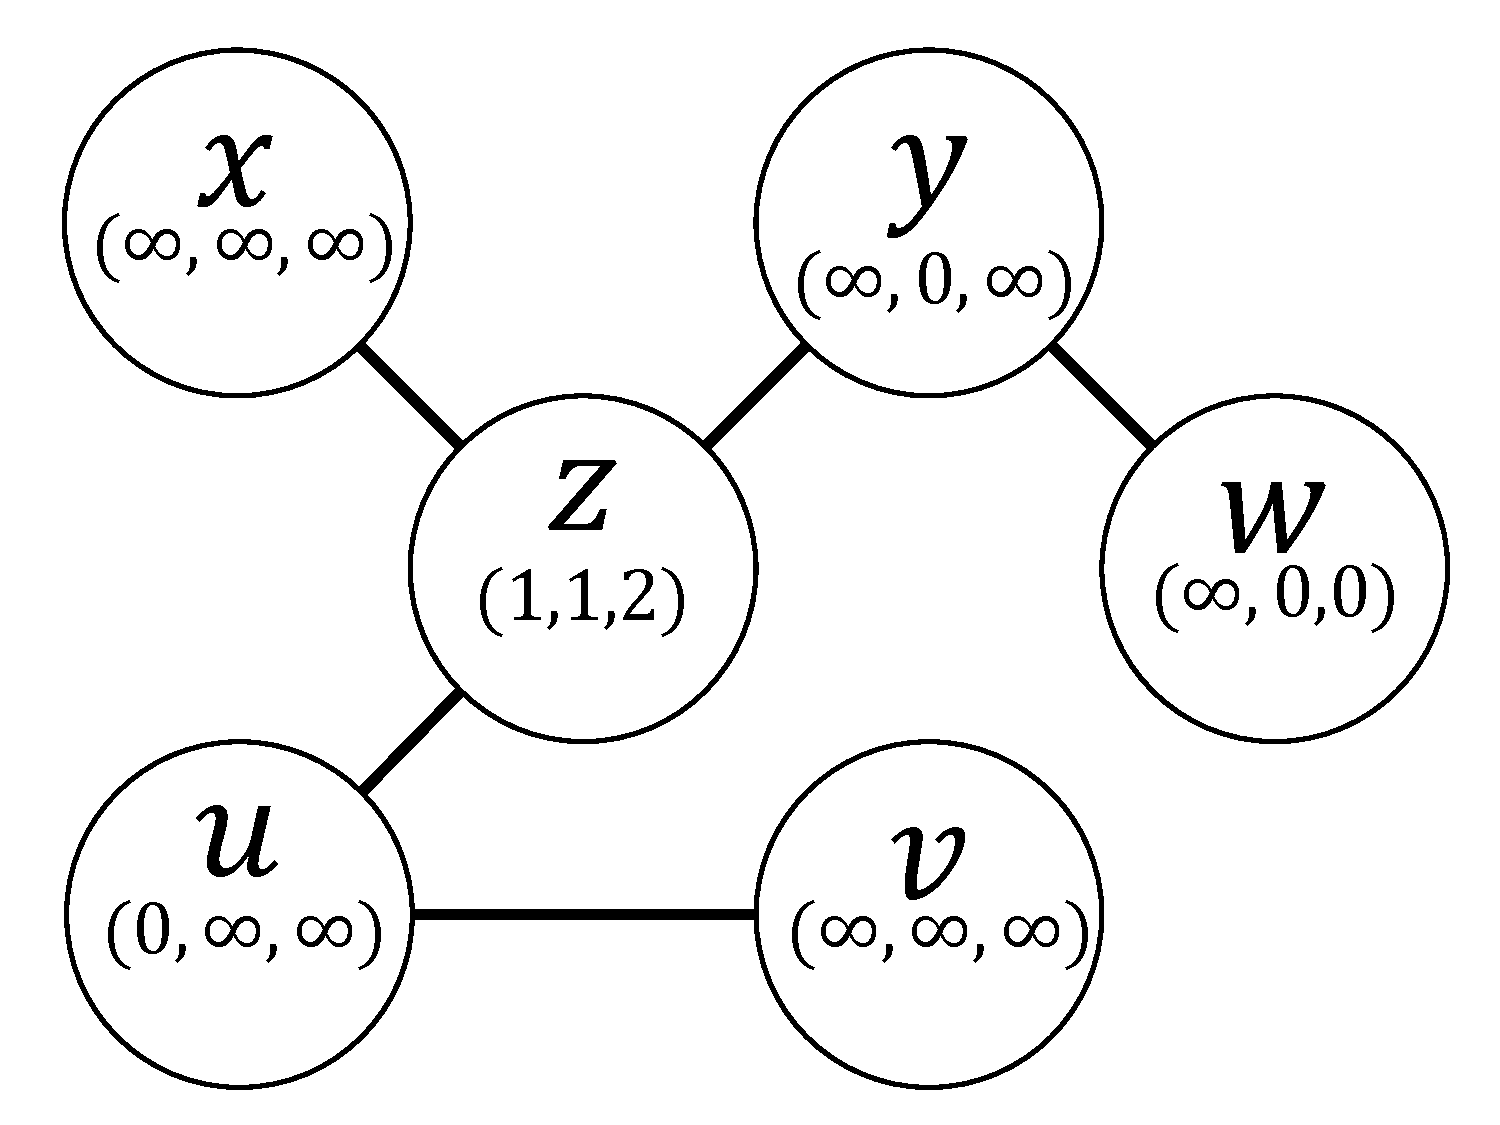
\includegraphics[width=0.5\textwidth]{figs/graph_example_1}
    \caption{Label distance vector after the first iteration}
    \label{fig:cand_step1}
\end{figure}

\begin{table}[H]
    \centering
    \begin{tabular}{|l|l|l|}
    \hline
      & SDS         & EQS         \\ \hline
    u & A           & $\emptyset$ \\ \hline
    v & $\emptyset$ & $\emptyset$ \\ \hline
    w & BC          & $\emptyset$ \\ \hline
    x & $\emptyset$ & $\emptyset$ \\ \hline
    y & B           & $\emptyset$ \\ \hline
    \end{tabular}
    \caption{SDS and EQS of each vertex after the first iteration}
    \label{tab:sds_step1}
\end{table}

\begin{table}[H]
    \centering
    \begin{tabular}{|l|l|}
    \hline
    Subspaces & Dominating candidate \\ \hline
    A         & $(u, dom)$            \\ \hline
    B         & $(w, dom), (y, dom)$            \\ \hline
    C         & $(w, dom)$            \\ \hline
    \end{tabular}
    \caption{Dominating candidate set of each $1$-dimensional subspace after the first iteration}
    \label{tab:cand_set_step1}
\end{table}

Consider the LinkedIn network represented by Table~\ref{tab:skill_sets} and Figure~\ref{fig:graph} as our running example. Again, we take $q$ as the query vertex. The labeled distance vectors of all vertices are originally initialized as ($\infty$, \dots, $\infty$). As shown in Figure~\ref{fig:cand_step1}, we start from the vertices with labels and mark the corresponding entries of the labeled distance vectors of those vertices as $0$. 
We add the label $A$ to $\mathit{SDS}_u$ because $u$ dominates the query vertex $q$ in dimension $A$. Table~\ref{tab:sds_step1} shows the $\mathit{SDS}$ and $\mathit{EQS}$ of all the vertices after the first iteration.
After the first iteration, since $u$ dominates $q$ in the $1$-dimensional subspace $A$, we add $(u, dom)$ to the dominating candidate set $\mathit{CAND}_A$ as shown in Table~\ref{tab:cand_set_step1}.

\begin{figure}[H]
    \centering
    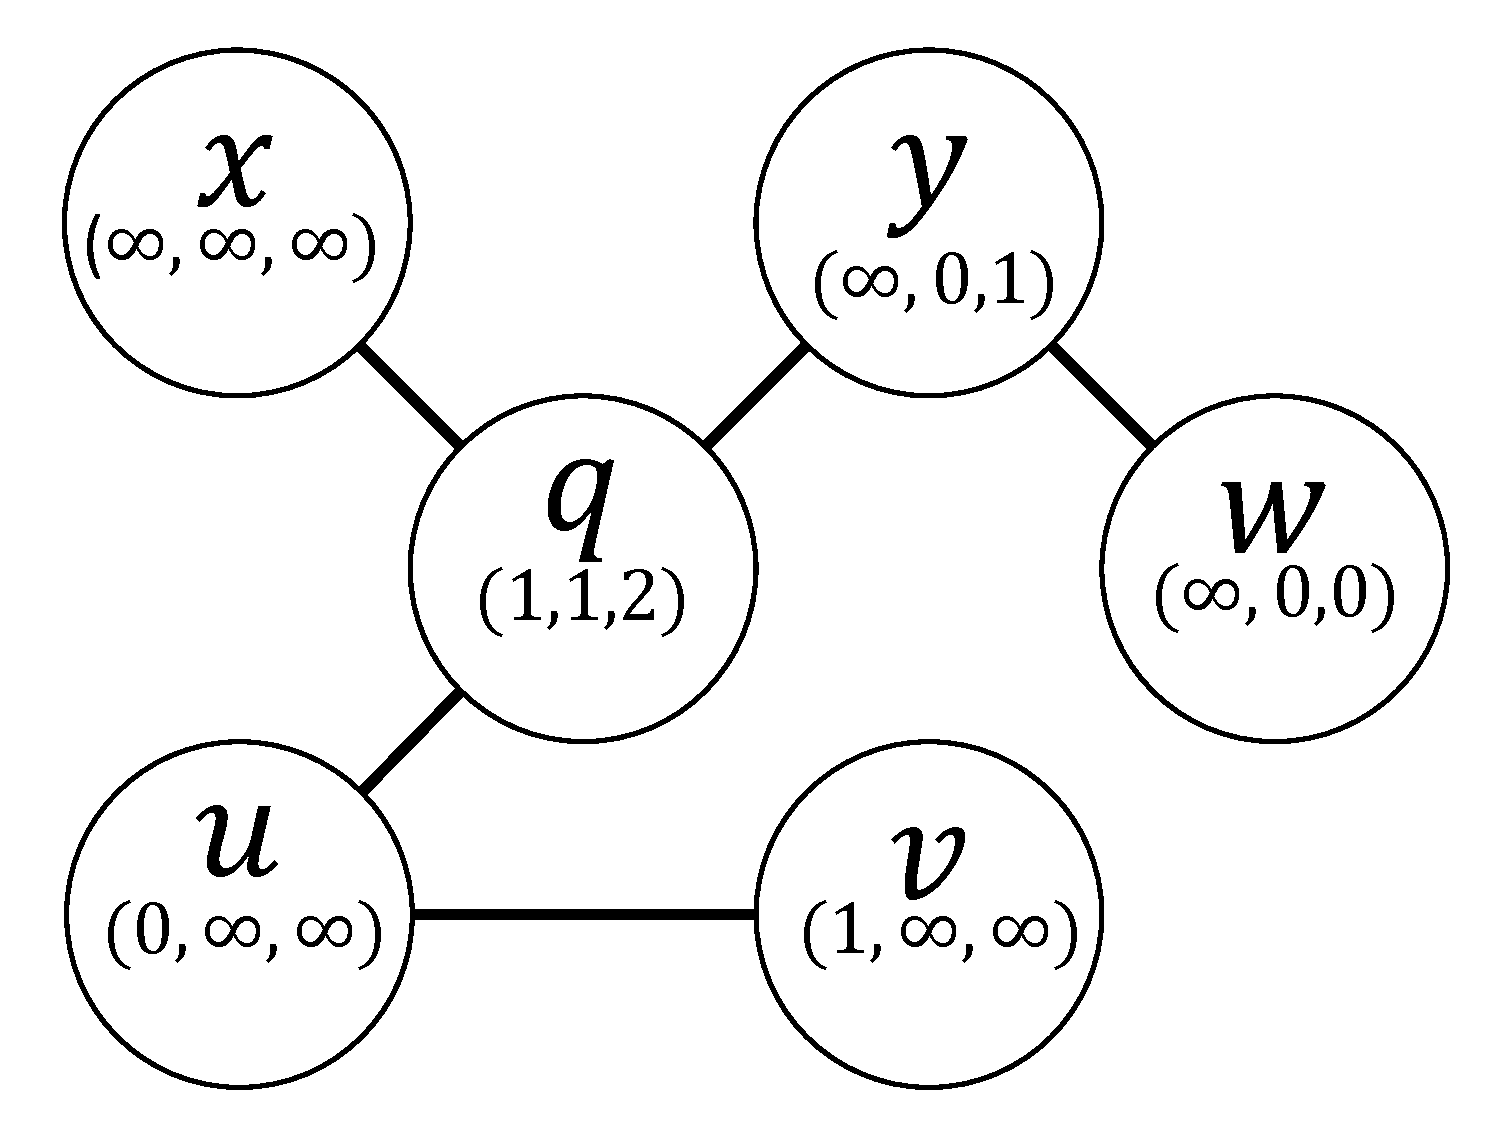
\includegraphics[width=0.5\textwidth]{figs/graph_example_2}
    \caption{Label distance vector after second iteration}
    \label{fig:cand_step2}
\end{figure}

\begin{table}[H]
    \centering
    \begin{tabular}{|l|l|l|}
    \hline
      & SDS         & EQS         \\ \hline
    u & A           & $\emptyset$ \\ \hline
    v & $\emptyset$ & A           \\ \hline
    w & BC          & $\emptyset$ \\ \hline
    x & $\emptyset$ & $\emptyset$ \\ \hline
    y & BC          & $\emptyset$ \\ \hline
    \end{tabular}
    \caption{SDS and EQS of each vertex after the second iteration}
    \label{tab:sds_step2}
\end{table}

\begin{table}[H]
    \centering

    \begin{tabular}{|l|l|}
    \hline
    Subspaces & Dominating candidate \\ \hline
    A         & $(u, dom), (v, eq)$            \\ \hline
    B         & $(w, dom), (y, dom)$            \\ \hline
    C         & $(w, dom), (y, dom)$            \\ \hline
    \end{tabular}
    \caption{Dominating candidate set of each $1$-dimensional subspace after the second iteration}
    \label{tab:cand_set_step2}
\end{table}


Then, we explore the graph in a breadth first manner. On the second iteration, as shown in Figure~\ref{fig:cand_step2}, we visit the neighbours of the vertices that were visited in the first iteration and update the corresponding entries of their labeled distance vectors. Table~\ref{tab:sds_step2} shows that subspace $A$ is added to $\mathit{EQS}_v$ because on the second iteration we update the distance between $v$ and label $A$ to $2$ which is equal to the distance between $q$ and label $A$. For the same reason, we add $(v, eq)$ to $\mathit{CAND}_A$ as shown in Table~\ref{tab:cand_set_step2}. It means that in $1$-dimensional subspace $A$, $v$ is equal to $q$ and it is still possible for $v$ to dominate $q$.

After two iterations, the process of building the dominating candidate sets of all $1$-dimensional subspace ends. The \emph{strictly dominating subspaces} and the \emph{equivalence subspaces} of all the vertices on graph are built. In Figure~\ref{tab:d_hops_distance}, we collect the $3$-hop labels by Breadth-First-Search and get the label vectors. By this point, if the value of label $l$ in the labeled distance vector of vertex $v$ is $\infty$, then it means the distance between label $l$ and vertex $v$ is longer than the distance between the label $l$ and the query vertex $q$.

\begin{table}[h]
    \centering
    \begin{tabular}{llll}
    \hline
    Distances & A & B & C \\ \hline
    $u$       & 0 & $\infty$ & $\infty$ \\ \hline
    $v$       & 1 & $\infty$ & $\infty$ \\ \hline
    $w$       & $\infty$ & 0 & 0 \\ \hline
    $x$       & $\infty$ & $\infty$ & $\infty$ \\ \hline
    $y$       & $\infty$ & 0 & 1 \\ \hline
    $q$       & 1 & 1 & 2 \\ \hline
    \end{tabular}
    \caption{Distances between each person and each skill in 2-hop}
    \label{tab:d_hops_distance}
\end{table}

Although some information is still missing (equal to $\infty$) in Table~\ref{tab:d_hops_distance}, we are still able to get the minimal skyline subspaces of $q$: $(A, B)$ and $(A, C)$ from the Table~\ref{tab:d_hops_distance}.

\section{Dominating Candidate Pruning}

In this section, we will introduce a way to prune the unnecessary vertices using the \emph{strictly dominating subspace}, $\mathit{SDS}$, and the \emph{equivalence subspace}, $\mathit{EQ}$ of the vertices.


\begin{lemma}
\label{ppt:prune_cand}
Given a vertex $u$, if there exists a vertex $v$, such that $(SDS_u \cup EQS_u \subseteq SDS_v \cup EQS_v) \wedge (SDS_u \subseteq SDS_v)$, and $(u, dom) \in \mathit{CAND}_\mathcal{B}$, then for any subspace $\mathcal{B}$, we have $(v, dom) \in \mathit{CAND}_\mathcal{B}$.
\end{lemma}

\begin{proof}
We prove this lemma by contradiction. Suppose there exists a subspace $\mathcal{B}$, such that $(u, dom) \in \mathit{CAND}_\mathcal{B}$, but $(v, dom) \not\in \mathit{CAND}_\mathcal{B}$. Then $(u, dom) \in \mathit{CAND}_\mathcal{B}$ implies that vertex $u$ dominates query vertex $q$ in subspace $\mathcal{B}$.
$(v, dom) \not\in \mathit{CAND}_\mathcal{B}$ implies that $v$ does not dominate query vertex $q$ in subspace $\mathcal{B}$. There are two possible cases that $v$ does not dominate $q$.

Case 1: The values of all dimensions in subspace $\mathcal{B}$ of $v$ are all equal to the values of $q$. Since $u$ dominates $q$ in subspace $\mathcal{B}$, in one of the dimensions of $\mathcal{B}$, the value of $u$ is less than $q$ , say dimension $c$. By the definition of \emph{strictly dominating subspace}, we have $c \in SDS_u$. We have $c \notin SDS_v$, since $v$ equals to $q$ in subspace $\mathcal{B}$. Therefore, $SDS_u \subseteq SDS_v$ and $SDS_u \not\subseteq SDS_v$, a contradiction.

Case 2: In one of the dimensions of subspace $\mathcal{B}$, say dimension $e$, vertex $v$ has a greater value than query vertex $q$. By the definitions of \emph{strictly dominating subspace} and \emph{equivalence subspace}, we have $e \notin SDS_v \cup EQS_v$. Since $u$ dominates $q$ in subspace $\mathcal{B}$ and $e \in \mathcal{B}$, the value of $u$ in dimension $e$ is less than or equal to the value of $q$ in dimension $e$. Thus, $e \in SDS_u$ or $e \in EQS_u$. Thus $e \in SDS_u \cup EQS_u$. Therefore, we have $SDS_u \cup EQS_u \not\subseteq SDS_v \cup EQS_v$, a contradiction.
\end{proof}


Subspace $\mathcal{B}$ is a skyline subspace if and only if $\mathit{CAND}_\mathcal{B}$ does not contain any vertices that dominate $q$ in subspace $\mathcal{B}$. As long as $\mathit{CAND}_\mathcal{B}$ contains one vertex, say $(w, dom)$ that dominates $q$, $\mathcal{B}$ is not a skyline subspace. We determine whether a subspace $\mathcal{B}$ is skyline subspace by checking whether there exists such a $(w, dom)$ that $(w, dom) \in \mathit{CAND}_\mathcal{B}$. By Lemma~\ref{ppt:prune_cand}, we notice that $(u, dom)$ always comes with the vertex $(v, dom)$. Thus, given a subspace $\mathcal{B}$, pruning $u$ from $\mathit{CAND}_\mathcal{B}$ does not affect the result of deciding whether the subspace $\mathcal{B}$ is a skyline subspace.


Given a point $u$, if we are able to find such a point $v$ that $(SDS_u \cup EQS_u \subseteq SDS_v \cup EQS_v) \wedge (SDS_u \subseteq SDS_v)$, by Lemma~\ref{ppt:prune_cand}, $u$ can be pruned from the \emph{dominating candidate sets} that $u$ belongs to.

How to find such a vertex $v$? One way to find such a $v$ is to enumerate all the vertices in the graph $G$ to check whether the statement $(SDS_u \cup EQS_u \subseteq SDS_v \cup EQS_v) \wedge (SDS_u \subseteq SDS_v)$ is true or not. It takes $O(n)$ time to determine whether a vertex $u$ can be pruned from its \emph{dominating candidate sets}.

In our thesis, we heuristically search for the vertex $v$ from the neighbours of the query vertex $q$. The intuition is that usually the neighbours of query vertex $q$ will have \emph{strictly dominating subspaces} with more dimensions, comparing to the vertices that are not the neighbours of query vertex. The reason is that for any label $D$, every vertex $w$ (except for $q$ itself) on the shortest path from the query vertex $q$ to the label $D$ has $w.D < q.D$. In other words, the \emph{strictly dominating subspaces} of the vertices on the shortest path must contain dimension $D$. Heuristically, a neighbour vertex of the query vertex $q$ is on multiple shortest paths from the query vertex $q$ to the labels.

For example, in Figure~\ref{fig:heuristic}, one of the neighbours $w$ is on the shortest paths from query vertex $q$ to label $D$, label $E$, and label $F$.
Thus, the neighbours of the query vertex $q$ tend to have \emph{strictly dominating subspaces} with multiple dimensions. In Figure~\ref{fig:heuristic}, we have $SDS_u=\{A, B\}, SDS_x=\{C\}, SDS_w=\{D, E, F\}$.
By Lemma~\ref{ppt:prune_cand}, the vertices enclosed by the solid line can be pruned by vertex $u$, the vertices enclosed by the dot line can be pruned by vertex $x$, and the vertices enclosed by the dash line can be pruned by vertex $w$.
We develop a $1$-hop pruning algorithm. In Algorithm~\ref{algo:pruning_graph}, $S$ contains all query vertex's neighbours. If both $SDS_u$ and $SDS_u \cup EQS_u$ are subsets of $SDS_v$ and $SDS_v \cup EQS_v$ ($v \in s$), respectively, then we prune $u$ from the \emph{dominating candidate sets}.


\begin{figure}[H]
    \centering
    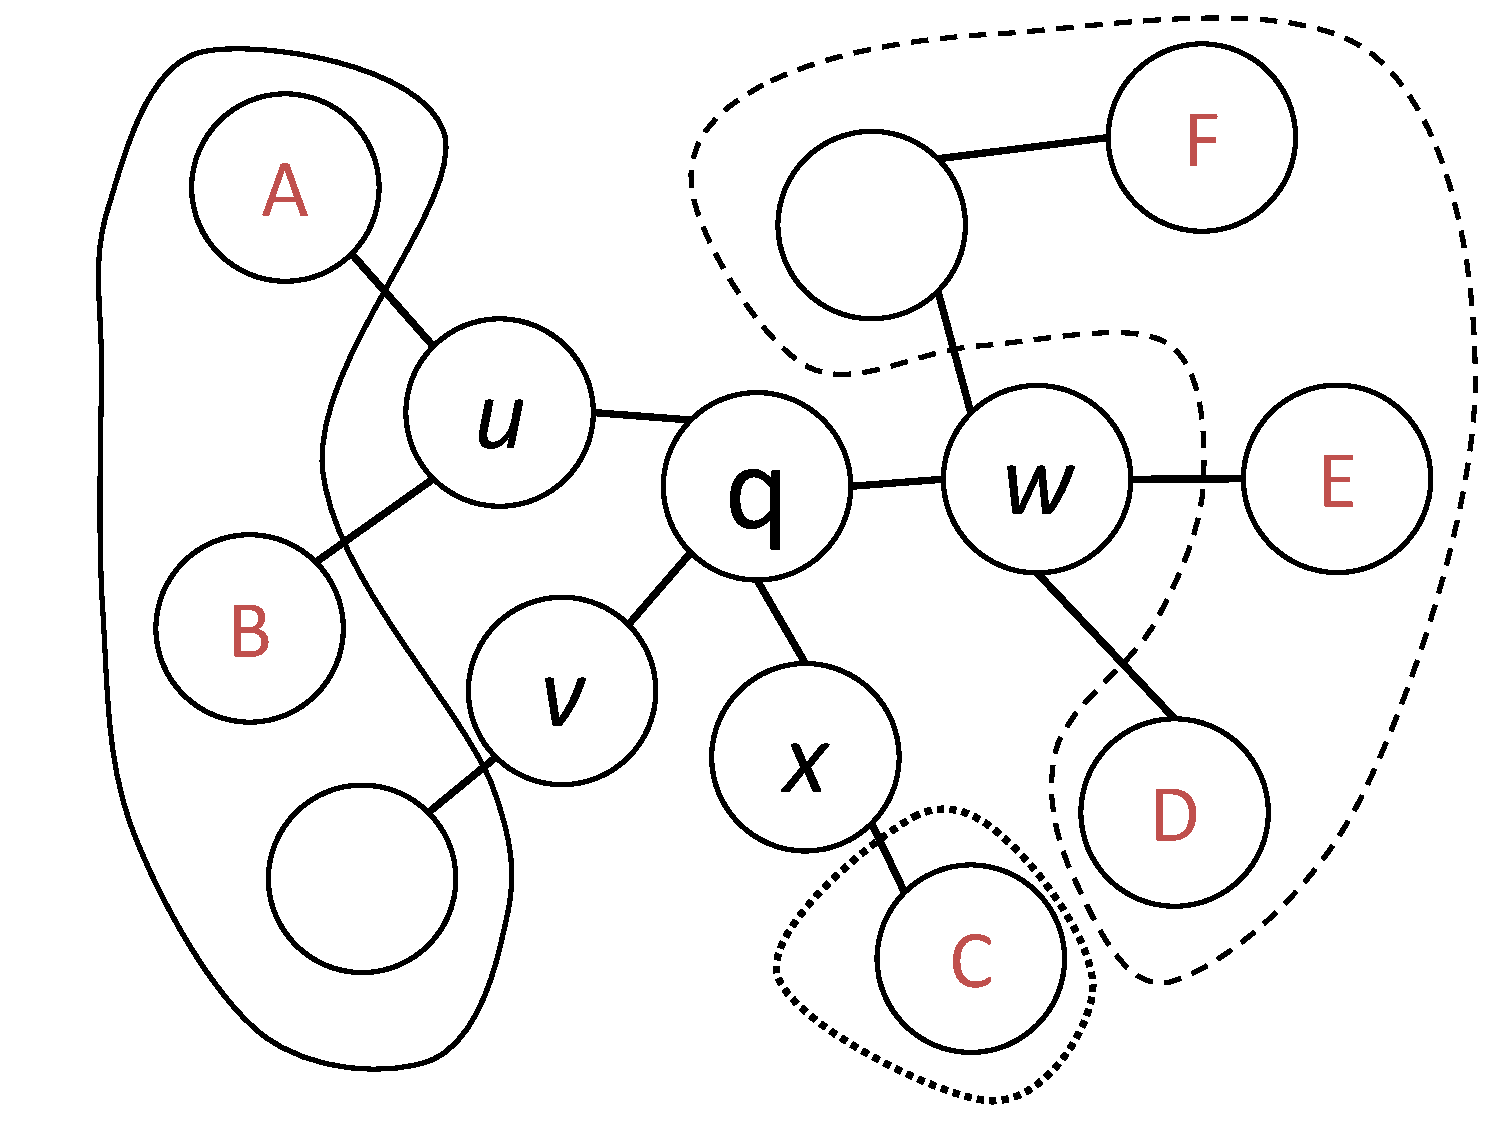
\includegraphics[width=0.6\textwidth]{figs/heuristic}
    \caption{Example of neighbours of query vertex $q$}
    \label{fig:heuristic}
\end{figure}

\begin{algorithm}[H]
  \caption{1-hop Pruning}
  \label{algo:pruning_graph}
  \begin{algorithmic}[1]
  \show\LOOP
    \REQUIRE Strictly Dominating Subspace $\mathit{SDS}$, Equivalence Subspace $\mathit{EQS}$, Dominating candidate $\mathit{CAND}$, query vertex $q$, graph $G=(V, E)$;
    \ENSURE Pruned Dominating candidate $\mathit{CAND}$;
    \STATE $S$ = $\left\{v|e(v, q) \in E \wedge (\forall u, e(u, q) \in E \wedge SDS_v \not\subset SDS_u)\right\}$
    
    \FORALL {$(l, dist)$ in $LV_q$}
        \FORALL {$u$ in $\mathit{CAND}_l$}
            \FORALL {$v$ in $S$}
                \IF {$u \not= v \wedge SDS_u \cup EQS_u \subseteq SDS_v \cup EQS_v \wedge SDS_u \subseteq SDS_v$}
                    \STATE delete $u$ from $\mathit{CAND}_l$
                \ENDIF
                
            \ENDFOR
        \ENDFOR
    \ENDFOR
  \end{algorithmic}
\end{algorithm}

\begin{table}[h]
    \centering
    \begin{tabular}{|l|l|l|l|}
    \hline
    Dim & $SDS$       & $EQS$       & $SDS \cup EQS$ \\ \hline
    $u$ & A           & $\emptyset$ & A              \\ \hline
    $v$ & $\emptyset$ & A           & A              \\ \hline
    $w$ & BC          & $\emptyset$ & BC             \\ \hline
    $x$ & $\emptyset$ & $\emptyset$ & $\emptyset$    \\ \hline
    $y$ & BC          & $\emptyset$ & BC             \\ \hline
    \end{tabular}
    \caption{The $SDS$ and $EQS$ of each vertex}
    \label{tab:SDS_EQS}
\end{table}

Table~\ref{tab:SDS_EQS} shows $SDS$ and $EQS$ of all vertices on the graph from Figure~\ref{fig:graph}. We can prune the some of the vertices from the \emph{dominating candidate set} according this table. By Lemma~\ref{ppt:prune_cand}, vertex $v$ can be pruned by $u$ and vertex $w$ can be pruned by $y$.

\begin{table}[h]
    \centering
    \begin{tabular}{lllll}
    \hline
    Distances & A & B & C & Pruned By\\ \hline
    $u$       & 0 & $\infty$ & $\infty$ &\\ \hline
    $v$       & 1 & $\infty$ & $\infty$ & $u$\\ \hline
    $w$       & $\infty$ & 0 & 0 & $y$\\ \hline
    $x$       & $\infty$ & $\infty$ & $\infty$ & $u$\\ \hline
    $y$       & $\infty$ & 0 & 1 & \\ \hline
    $q$       & 1 & 1 & 2 &\\ \hline
    \end{tabular}
    \caption{Label distance vector after 1-hop pruning}
    \label{tab:lv_pruned}
\end{table}

\begin{table}[H]
    \centering
    \begin{tabular}{|l|l|}
    \hline
    Subspaces & Dominating candidate \\ \hline
    A         & $(u, dom)$            \\ \hline
    B         & $(y, dom)$            \\ \hline
    C         & $(y, dom)$            \\ \hline
    \end{tabular}
    \caption{Pruned dominating candidate set of $1$-dimensional subspace}
    \label{tab:dom_cand_pruned}
\end{table}

Table~\ref{tab:lv_pruned} shows that $v$ and $x$ are pruned by $u$. Also, $y$ is pruned by $w$. Table~\ref{tab:lv_pruned} shows the vertices to be pruned and their labeled distance vectors. Although $w$ seems to be better than $y$ (because $w$ dominates $y$), vertex $w$ is pruned by vertex $y$ because both vertices $y$ and vertex $w$ have the same \emph{SDS} and \emph{EQS} and $y$ is a $1$-hop neighbour of the query vertex $q$. Table~\ref{tab:dom_cand_pruned} shows the dominating candidate sets of the $1$-dimensional subspaces after the $1$-hop neighbour pruning.

\subsection{Dominating Candidate Sets for Multi-dimensional Subspaces}

We generate the dominating candidate set on multi-dimensional subspaces by intersecting the dominating candidate sets of subspaces with lower dimensionality. The \emph{CAND} set intersection operation is computed in the following way:
Given subspaces $\mathcal{A}$ and $\mathcal{B}$,
\begin{align*} 
\label{cmpt:intersection}
W &= \{(u, dom) |\forall u, (u, dom)\in \mathit{CAND}_\mathcal{A} \wedge (u, eq)\in \mathit{CAND}_\mathcal{B} \} \\
X &= \{(u, dom) |\forall u, (u, eq)\in \mathit{CAND}_\mathcal{A} \wedge (u, dom)\in \mathit{CAND}_\mathcal{B} \} \\
Y &= \{(u, dom) |\forall u, (u, dom)\in \mathit{CAND}_\mathcal{A} \wedge (u, dom)\in \mathit{CAND}_\mathcal{B}\} \\
Z &= \{(u, eq) |\forall u, (u, eq)\in \mathit{CAND}_\mathcal{A} \wedge (u, eq)\in \mathit{CAND}_\mathcal{B} \} \\
\mathit{CAND}_{\mathcal{A} \cup \mathcal{B}} &= W \cup X \cup Y \cup Z
\end{align*}

For example, we consider two dominating candidate sets $\mathit{CAND}_\mathcal{A} = \left\{(u, dom)\right\}$ and $\mathit{CAND}_\mathcal{B} = \left\{(u, eq)\right\}$. We want to compute the CAND intersection of these two dominating candidate sets $\mathit{CAND}_{\mathcal{A} \cup \mathcal{B}}$. 
Both $\mathit{CAND}_\mathcal{A}$ and $\mathit{CAND}_\mathcal{B}$ contain the element $u$. In this example, vertex $u$ dominates query vertex $q$ in subspace $\mathcal{A}$ and vertex $u$ is equal to query vertex $q$ in subspace $\mathcal{B}$. 
Therefore, vertex $u$ dominates query vertex $q$ in the subspace $\mathcal{A} \cup \mathcal{B}$ because $u$ is less than $q$ in at least one dimension of $\mathcal{A} \cup \mathcal{B}$ ($u$ dominates $q$ in $\mathcal{A}$). 


\subsection{Buttom-up Subspace Eumeration}

In this section, we introduce a buttom-up algorithm to compute the dominating candidate sets from $1$-dimensional subspaces to $n$-dimensional subspaces.
This algorithm is inspired by the Apriori algorithm for mining association rules~\cite{agrawal1996fast}. A similar buttom-up algorithm has also been used in enumerating different subspaces in subspace clustering problem~\cite{agrawal1998automatic}.

\begin{property}
If in a k-dimensional subspace $\mathcal{B}$, $\mathit{CAND}_\mathcal{B}$ contains a set of vertices $S$, then in any (k-1)-dimensional projection $\mathcal{C}$ of $\mathcal{B}$, $\mathit{CAND}_\mathcal{C}$ also contains the set of vertices $S$.
\end{property}

\begin{proof}
If a vertex $v$ is in $\mathit{CAND}_\mathcal{B}$, where space $\mathcal{B}$ is a k-dimensional subspace, then the vertex $v$ is not greater than query vertex $q$ in any dimension of space $\mathcal{B}$. For any (k-1)-dimensional projection $\mathcal{C}$ of $B$, the vertex $v$ is also is not greater than query vertex $q$ in any dimension of projection $\mathcal{C}$. Therefore, in projection $\mathcal{C}$, $\mathit{CAND}_\mathcal{C}$ contains the vertex $v$.
\end{proof}

The algorithm computes the dominating candidate sets from one dimensional subspaces to $n$-dimensional subspaces. We already introduce an algorithm to compute the dominating candidate sets on all $1$-dimensional subspaces. Having all the dominating candidate sets on all $(k-1)$-dimensional subspaces, we are able to construct the non-empty dominating candidate sets on $k$-dimensional subspaces $L_k = \left\{\mathcal{A} \cup \left\{b\right\} | \mathcal{A} \in L_{k-1} \wedge b \in \bigcup L_{k-1} \wedge b \notin \mathcal{A} \right\}$. $L_k$ is the set of $k$-dimensional subspaces on which the dominating candidate sets are non-empty.

\begin{algorithm}[H]
  \caption{Subspace Eumeration}\label{algo:blah}
    \begin{algorithmic}[1]
  \show\LOOP
    \REQUIRE Dominating candidate $\mathit{CAND}$ of all one dimension subspaces in $LV_q$;
    \ENSURE A set of subspaces $SUB$ where query vertex $q$ is a skyline point;
        \FORALL {$\left(l, dist\right)$ in $LV_q$}
            \STATE if $\exists u, (u, dom)\in \mathit{CAND}_l$, add $l$ to $SUB$, else add $l$ to $L_1$
        \ENDFOR
        \STATE $k$ = 2
        \WHILE {$L_{k-1} \not= \emptyset$}
            \STATE $L_k = \left\{\mathcal{A} \cup \left\{b\right\} | \mathcal{A} \in L_{k-1} \wedge b \in \bigcup L_{k-1} \wedge b \notin \mathcal{A} \right\}$
            \FORALL{$\mathcal{C}$ in $L_k$}
                \FORALL{(k-1)-projection $\mathcal{S}$ of $\mathcal{C}$ do}
                    \IF {$\mathcal{S} \notin L_{k-1}$}
                        \STATE delete $\mathcal{C}$ from $C_k$
                    \ENDIF
                \ENDFOR
            \ENDFOR
            
            \FORALL{$\mathcal{C}$ in $L_k$}
                \STATE Let $b$ be the last element in $c$
                \STATE $CAND_\mathcal{C}$ = $CAND_b \cap CAND_{\mathcal{C}-\left\{b\right\}}$
                \STATE if $CAND_l$ is empty, add $l$ to $SUB$, else add $l$ to SUB
            \ENDFOR
            
            \STATE $k$ = $k$ + 1
        \ENDWHILE
        \RETURN SUB
  \end{algorithmic}
\end{algorithm}

We still take the LinkedIn network in Table~\ref{tab:skill_sets} and Figure~\ref{fig:graph} as our running example. By running the \emph{set enumeration} algorithm we get the \emph{dominating candidate sets} in all subspaces in Table~\ref{tab:sub_dom_cand_pruned}.

\begin{table}[H]
    \centering
    \begin{tabular}{|l|l|l|}
    \hline
    Subspaces & Dominating Candidates & Generated by \\ \hline
    A         & $(u, dom)$  &              \\ \hline
    B         & $(w, dom)$  &              \\ \hline
    C         & $(w, dom)$  &              \\ \hline
    AB        & $\emptyset$           & $A \cap B$   \\ \hline
    AC        & $\emptyset$           & $A \cap C$   \\ \hline
    BC        & $(w, dom)$            & $B \cap C$   \\ \hline
    \end{tabular}
    \caption{Dominating candidate in all subspaces}
    \label{tab:sub_dom_cand_pruned}
\end{table}

As shown in Table~\ref{tab:sub_dom_cand_pruned}, $\mathit{CAND}_{BC}$ is computed by $\mathit{CAND}_{B} \cap \mathit{CAND}_{C}$, $\mathit{CAND}_{AB}$ is computed by $\mathit{CAND}_{A} \cap \mathit{CAND}_{B}$ and $\mathit{CAND}_{AC}$ is computed by $\mathit{CAND}_{A} \cap \mathit{CAND}_{C}$. In this example, $\mathit{CAND}_{BC} = \mathit{CAND}_B \cap \mathit{CAND}_C = \left\{(w, dom)\right\}$, $\mathit{CAND}_{AB} = \emptyset$ and $\mathit{CAND}_{AC} = \emptyset$.
The query vertex $q$ is a skyline point on subspaces $AB$ and $AC$ because their dominating candidate sets are all empty.
